%!TEX root = ../../thesis.tex
\renewcommand{\chapterpath}{\allchapterspath/planning}
\renewcommand{\imgpath}{\chapterpath/img}

\chapter{Planning upon Uncertainty}
\label{chapter:planning}
\minitoc

Context - Why now: we shown that we can solve the problem but did not considered the problem of planning

Need - Why the reader: the planning has been shown to be an important aspect of most online real world learning system, 

Task - Why me: we investigated the problem of uncertainty in our problem

Object- Why this chapter: We start by providing an intuition on what are the sources of uncertainty inherent to our problem. Describe a metric that is able to measure it and show on simulated experiment that this method is more efficient than several standard ones.

Findings - What: We identified two sources of uncertainty in for our problem and combined them into one efficient metrics that reduce to other method if the mapping between signal and meaning was known

Conclusions - So what: We can improve the learning efficiency of such a system that become aware of the information it misses or it miss model and can actively try to recover from this.

Perspectives - What now: how does it apply to a real word complex scenario. actually useful for some person that can't use button and where signal are never the same, where some universal classifier does no exist.

%%%%%%%%%%%%%%%%%%%%%%%%%%%%%%%%%%%%%%%%%%%%%%
%%%%%%%%%%%%%%%%%%%%%%%%%%%%%%%%%%%%%%%%%%%%%%
%%%%%%%%%%%%%%%%%%%%%%%%%%%%%%%%%%%%%%%%%%%%%%
%%%%%%%%%%%%%%%%%%%%%%%%%%%%%%%%%%%%%%%%%%%%%%
%%%%%%%%%%%%%%%%%%%%%%%%%%%%%%%%%%%%%%%%%%%%%%
\section{Problem formulation and assumptions}

Our algorithm is able to identify a task among a set of possible tasks. To do so it has to explore regions allowing to disambiguate among task hypotheses. There are several efficient model-based reinforcement learning exploration methods that add an exploration bonus for states that might provide more learning gains. Several theoretical results show that these approaches allow to learn tasks efficiently \cite{brafman2003r,kolter2009near}. We define an uncertainty measure and use model-based planning to select sequences of actions that guide the agent towards states that better identify the desired task.

Our algorithm is based on comparing the expected classification rate between different task hypotheses. Therefore, to disambiguate between hypotheses, it has to collect data which are likely to affect differently the dataset quality of competing hypotheses. As we have access to the optimal policies of each task, we can choose for a given task an action in a given state and predict to receive a ``correct'' or ``wrong'' label. Such label is linked to a signal generation model (parameterized by $\theta^{ML}_{\xi_t}$) which differs from task to task, and to the optimal action at that particular state. A state-action pair where the optimal actions and the signal models are the same for all hypotheses is unlikely to tell them apart and will be less informative that any other state-action where either optimal actions or signal models differ between hypotheses.

Thus, we define a measure of global uncertainty $U(s,a)$ that is higher when, for a given state-action, there is a high incongruity between either optimal actions or signal models. For this we compute a similarity matrix $S$ where each element $S_{ij}(s,a)$ corresponds to the similarity of the distributions of signals associated to the expected label from tasks $i$ and $j$ if action $a$ is performed in state $s$. The final uncertainty value $U(s,a)$ is computed as the opposite of the weighted sum of the similarity matrix elements:
%
\begin{eqnarray}
U(s,a) &=& - \sum_{i = 1}^{T} \sum_{j = 1}^{T} S_{ij}(s,a) p(\xi_i)p(\xi_j)
\end{eqnarray}
%
Computing the similarity between two Gaussian distributions for all state-action pairs was not feasible in real time. In order to improve computation efficiency we do not rely on a precise metric between Gaussian distributions and only consider the similarity between their means (empirical tests did show that this approximation does not impact the results).

Computed for each state and action, this measure is then used as an exploration bonus, whereas we switch to a pure exploitation of the task after reaching the desired confidence level~$\beta$.

%%%%%%%%%%%%%%%%%%%%%%%%%%%%%%%%%%%%%%%%%%%%%%
%%%%%%%%%%%%%%%%%%%%%%%%%%%%%%%%%%%%%%%%%%%%%%
%%%%%%%%%%%%%%%%%%%%%%%%%%%%%%%%%%%%%%%%%%%%%%
%%%%%%%%%%%%%%%%%%%%%%%%%%%%%%%%%%%%%%%%%%%%%%
%%%%%%%%%%%%%%%%%%%%%%%%%%%%%%%%%%%%%%%%%%%%%%
\section{What is different with our setup that should be exploited, visual example}

%%%%%%%%%%%%%%%%%%%%%%%%%%%%%%%%%%%%%%%%%%%%%%
%%%%%%%%%%%%%%%%%%%%%%%%%%%%%%%%%%%%%%%%%%%%%%
%%%%%%%%%%%%%%%%%%%%%%%%%%%%%%%%%%%%%%%%%%%%%%
%%%%%%%%%%%%%%%%%%%%%%%%%%%%%%%%%%%%%%%%%%%%%%
%%%%%%%%%%%%%%%%%%%%%%%%%%%%%%%%%%%%%%%%%%%%%%
\section{How do we exploit it}

refer to the video I did

After several interaction with the user, our algorithm is able to identify a task among a set of possible tasks. To do so it has to explore regions that allow to disambiguate among hypothesis. There are several efficient model-based reinforcement learning exploration methods that add an exploration bonus for states that might provide more learning gains. Several theoretical results show that these approaches allow to learn tasks efficiently \cite{brafman2003r,kolter2009near}. We define an uncertainty measure and use model-based planning to select sequences of actions that guide the agent toward states that better identify the desired task.

To solve our problem we need to identify simultaneously the task and how to interpret teaching signals. To do so it has to explore regions that allow to disambiguate among hypothesis. There are several efficient model-based reinforcement learning exploration methods that add an exploration bonus for states that might provide more learning gains. Several theoretical results show that these approaches allow to learn tasks efficiently \cite{brafman2003r,kolter2009near}. We define an uncertainty measure and use model-based planning to select sequences of actions that guide the agent toward states that better identify the desired task.

In order to exemplify the specificity of our problem in terms of planning we present a simple experiment and compare the effect of different action selection strategies. In this scenario, the agent is in a T world with 7 states and can perform 4 actions (right, left, up, and down). The goal of the agent is to reach one of the two edges of the T world (see figure \ref{fig:planningExplained} top), the one the user has in mind. After each agent's move, the user assesses the correctness of the agent action by providing a two dimensional teaching signal. The system then assign a label to each signal according to each hypothesis. The result of the labeling process is display as colored dot in figure \ref{fig:planningExplained} (a, b, and c), where the left part corresponds to hypothesis 1 and the right part to hypothesis 2.

\begin{figure}[!ht]
  \centering
      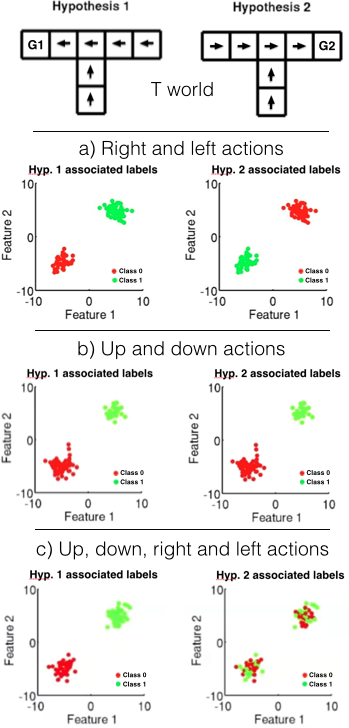
\includegraphics[width=0.6\columnwidth]{\imgpath/planning_explained.png}
      \caption{A ``T'' world scenario and the interpretation results for different planning strategies. The agent should reach either of the two edges of the T world (marked with the letter ``G''). The arrows represent the optimal policy. For each move it receives unlabeled two dimensional teaching signal which are interpreted according to each hypothesis. a) shows the interpretation results if the agent only perform right and left action in the top of the T world, b) shows the results when the agent only perform up and down action in the trunk of the T, and c) shows results for an agent performing all possible actions.}
    \label{fig:planningExplained}
\end{figure}

If the agent knew how to interpret the signal, i.e. which signal correspond to correct and incorrect feedback, the optimal action to differentiate between the two hypothesis would be to perform right and left actions in the top part of the T. However in our problem the classifier is not given and the agent is building a different model for each hypothesis. As a results, we end up with two opposite interpretations of the user signal, which are both as valid (see figure \ref{fig:planningExplained}a) and do not allow to differentiate between hypothesis.

Considering that the agent does not know the signal to meaning classifier, a sensitive option is to select action that allow to unequivocally identify the model. In our scenario taking only up and down actions in the trunk of the T leads to identical interpretation for each hypothesis (see figure \ref{fig:planningExplained}b). However this method do not allow to disambiguate between hypothesis and in most setting, such as the grid world we consider later, there is no state-action pair leading to unequivocal interpretations.

For our kind of problem the agent can not just try to differentiate hypothesis by finding state-action pair where expected feedback differs but should also collect data to build a good model or at least invalidate other models. Can we find a measure of uncertainty that account for both? Going back to figure \ref{fig:planningExplained} (a and b), we understand that, to differentiate hypothesis in situation a) the best actions to perform are up and down in the T trunk while in situation b) the best actions to perform are right and left in the top part of the T. This correspond to the uncertainty in the signal space. In the case of a) when going left both hypothesis agree that they will receive a signal in the top right part of the feature space even if they disagree on its meaning. However for action down, both hypothesis agree they should receive a signal of meaning ``incorrect'' but disagree on the expected location of such signal in the feature space. In the case of b) when going up both hypothesis agree they will receive a signal in the top right part of the feature space and agree on its meaning. However for action left, both hypothesis disagree about the meaning of signal they should receive and as both share the same model of the signal they expect signal in different location of the feature space.

Estimating uncertainty in the signal space is in practice too costly as it requires to compute, for every state-action pair, the overlap between many continuous distributions weighted by their respective expected contribution. Following the discussion presented in previous section, we will rely on our pseudo-likelihood metric. As we cannot predict, neither control, the signal we will receive for a particular state-action, we will rely on our past history of signal and compute the expected joint probability based on previously experienced signals.

To differentiate between tasks, our algorithm computes the probability that expected labels $l^{\xi_t}$ equals predicted labels $l^{\theta^{\xi_t}}$. In order to find which task is the correct one, we need to explore the state space where this value differs between likely hypothesis. As we cannot predict, neither control, the signal we will receive for a particular state-action, we will rely on our past history of signal and compute the expected joint probability based on previously experienced signals.

We note $J^{\xi_t}(s,a,e) = p(e | \xi_t, \theta, s, a)$ (see eq.\ref{eq:pseudo1}) and $J^{\xi}(s,a,e)$ the vector $[J^{\xi_1}(s,a,e), \ldots, J^{\xi_T}(s,a,e)]$.

The uncertainty of one state-action pair given a signal $e$ is computed as the weighted variance of the joint probability predictions with weights $W_{i}^{\xi} = [W^{\xi_1}, \ldots, W^{\xi_T}]$.
\begin{eqnarray}
U(s,a|e) = weightedVariance(J^{\xi}(s,a,e), W^{\xi})
\label{eq:planningOneSignal}
\end{eqnarray}

The uncertainty for a state-action pair is given by:
\begin{eqnarray}
U(s,a) & = & \int_{e} U(s,a|e) p(e) de
\end{eqnarray}
which we approximate by summing values of $U(s,a|e)$ for different signals $e$:
\begin{eqnarray}
U(s,a) & \approx & \sum_{e} U(s,a|e) p(e)
\label{eq:planning}
\end{eqnarray}

Our measure of global uncertainty $U(s,a)$ will be higher when, for a given state-action there is an high incongruity of expectation between each hypothesis and according to their current importance. 

This measure is then used as a classical exploration bonus method. We will switch to a pure exploitation of the task after reaching the desired confidence level.

Interestingly this approach generalizes over other active sampling method \cite{lopes2009active}, if the classifier is known, equation \ref{eq:planningOneSignal} reduces to the one presented in \cite{macl11simul} and is no longer dependent on signal $e$. As our uncertainty function combines uncertainty on both signal and task space, when former is known, the latter becomes the sole source of ambiguity.


%%%%%%%%%%%%%%%%%%%%%%%%%%%%%%%%%%%%%%%%%%%%%%
%%%%%%%%%%%%%%%%%%%%%%%%%%%%%%%%%%%%%%%%%%%%%%
%%%%%%%%%%%%%%%%%%%%%%%%%%%%%%%%%%%%%%%%%%%%%%
%%%%%%%%%%%%%%%%%%%%%%%%%%%%%%%%%%%%%%%%%%%%%%
%%%%%%%%%%%%%%%%%%%%%%%%%%%%%%%%%%%%%%%%%%%%%%
\section{Method}

In the subsequent analysis, we assume that a trainer provides feedback for the actions taken by a learner. Specifically, we consider the user is delivering signals that can be mapped into binary feedback: correct $c$ and incorrect $w$. 

\subsection{World and Task}
We consider a 5x5 grid world, where an agent can perform five different discrete actions: move up, down, left, right, or a stop action. The user goal is to teach the agent to reach one of the $25$ discrete positions which represent the set of possible tasks (unknown to the agent). We thus consider that the agent has access to 25 different task hypothesis (one with goal location at each of the cells). We use \textit{Markov Decision Processes} (MDP) to represent the problem \cite{sutton1998reinforcement}. From a given task $\xi$, represented as a reward function, we can compute the corresponding policy $\pi^{\xi}$ using, for instance, Value Iteration \cite{sutton1998reinforcement}. The policies allow us to interpret the teaching signals with respect to the interaction protocol defined. For the current work we will consider the user is providing feedback on the agent action. We define $p(l | \xi, s, a)$ as:

\begin{equation*}
    p(l | \xi, s, a) = 
    \begin{cases}
    1-\alpha               & if~a = \argmax_a \pi^{\xi}(s,a)\\
        \alpha             & \text{otherwise}\\
   \end{cases}
\end{equation*}
with $\alpha$ modeling the expected error rate of the user. 
% We use $\alpha = 0.1$.

\subsection{Signal properties and classifier}

We aim at applying this algorithm to error-related potentials (ErrPs) for EEG-based BCI applications. These signals are generated in the user´s brain after s/he assesses actions performed by an external agent \cite{chavarriaga2010learning}, where correct and erroneous assessments will elicit different brain signals. Past approaches have already demonstrated that these signals can be classified online with accuracies of around 80\% and translated into binary feedback, thanks to a prior calibration session that lasts for 30-40 minutes \cite{chavarriaga2010learning, iturrate2013task}.

Following the literature \cite{blankertz2010single}, we will model the signals using independent multivariate normal distributions for each class, $\mathcal{N}(\mu_c, \Sigma_c), \mathcal{N}(\mu_w, \Sigma_w)$. With $\theta$ the set of parameters $\{\mu_c, \Sigma_c,\mu_w, \Sigma_w\}$. Given the high dimensionality of the problem we will also need to regularize. For this we apply shrinkage to the covariance matrix ($\lambda = 0.5$) and compute the value of the marginal pdf function using a noninformative (Jeffrey's) prior [\cite{gelman2003bayesian}, p88]:

\begin{eqnarray}
p(e|\theta, l) & = & t_{n-d}(e | \mu_l,\frac{\Sigma_l (n+1)}{n(n-d)})
\label{eq:prior}
\end{eqnarray}
where $\theta$ represents the probability distribution over mean and covariance, $n$ is the number of signal, $d$ is the dimensionality, $\mu_l$ and $\Sigma_l$ the ML estimates of mean and covariance for the signals of class $l$.

\subsection{Task Achievement}

A task is considered completed when a confidence level as been reached for this task and the agent is located at the task associated state. If the state is the one intended by the user it is a success. Whatever the success or failure of first task, the user selects a new state randomly, the agent resets task likelihoods, propagates the believed labels, and teaching start again. At no point the agent has access to a measure of its performance, it can only refer to the unlabeled signals.


\subsection{Evaluation scenarios}

Two different evaluation scenarios were tested with two different types of signals: artificial datasets, and real ErrP datasets recorded from previous experiments \cite{iturrate2013task}.

\paragraph{Artificial datasets}
The goal of this evaluation was to analyze the feasibility of learning a task from scratch in a 5x5 grid world. 
%
The artificial dataset was composed of two classes, with 1000 examples per class. Each example was generated by sampling from a normal distribution with a covariance matrix of diagonal 1 and mean selected randomly. The datasets were generated while varying two factors: (i) the dimensionality of the data, where 2, 5, 10 and 30 features were tested; and (ii) the quality of the dataset, measured in terms of the ten-fold accuracy a linear classifier would obtain. 

Once the datasets were generated, two different evaluations were performed: (i) the goodness of our proposed planning strategy versus a) random action selection, b) greedy action selection, and c) a task-only uncertainty based method; (ii) the time required by the agent to learn the first task (i.e. to reach the first target), and (iii) the number of tasks that can be learned in 500 iterations.

\paragraph{EEG datasets}
Once the algorithm was evaluated with artificial datasets, we tested the feasibility of the proposed self-calibration approach using real ErrP datasets. The objective of this analysis is to study the scalability of our method to EEG data, which may have different properties than our artificial dataset. 

Following previous studies, the ErrP features were extracted from two fronto-central channels (FCz and Cz) within a time window of $[200,700]$ ms (being 0 ms the action onset of the agent) and downsampled to $32$ Hz. This leaded to a vector of $34$ features \cite{iturrate2013task}.

\paragraph{Comparison with calibration methods}
In order to show the benefit of learning without explicit calibration, we compare our method with the standard supervised BCI calibration procedure. In this calibration procedure, which can last for up to 40 minutes, the experimenter needs to record enough data from the user from several offline runs, where the user is not controlling the agent but just passively assessing its actions.
%
Following the literature on ErrPs \cite{chavarriaga2010learning,iturrate2013task} our training data will consist of 80 percent of positive examples (associated to a correct feedback) and 20 percent of negative examples (associated to an incorrect feedback). Our proposed algorithm is compared with different (but standard) sizes of calibration datasets: 200, 300 and 400 examples.

\subsection{Settings}

We used $\alpha = 0.1$, $\beta = 0.9$. For dataset of dimension $d$, we started computing likelihoods after $d+10$ steps as equation \ref{eq:prior} requires at least $d+1$ samples and to allow for cross validation. For the planning (eq. \ref{eq:planning}) we selected randomly $20$ signals from $D_i$.

%%%%%%%%%%%%%%%%%%%%%%%%%%%%%%%%%%%%%%%%%%%%%%
%%%%%%%%%%%%%%%%%%%%%%%%%%%%%%%%%%%%%%%%%%%%%%
%%%%%%%%%%%%%%%%%%%%%%%%%%%%%%%%%%%%%%%%%%%%%%
%%%%%%%%%%%%%%%%%%%%%%%%%%%%%%%%%%%%%%%%%%%%%%
%%%%%%%%%%%%%%%%%%%%%%%%%%%%%%%%%%%%%%%%%%%%%%
\section{Results}


We present most of the results in terms of the quality of the dataset, measured as the ten-fold classification accuracy that a calibrated signal classifier would obtain. Each simulation, was run 100 times using different sampled datasets, and their associated box plots \cite{mcgill1978variations} were computed. For each boxplot, colored bars show the interquartile range (between 25th and 75th percentile), and the median and the mean are marked as a horizontal line and a colored dot respectively. Additionally, the two ``whiskers'' show the 5th and 95th percentiles, black crosses are considered as outliers. 


\subsection{Artificial Datasets}
The first objective is to study the impact of the exploration approach proposed in Section \ref{sec:planning}. The second is to evaluate performances and robustness with respect to dimension and qualities of datasets. 

\paragraph{Planning Methods}
Figure \ref{fig:planning} compares the number of steps (with maximum values of 500 steps) needed to identify the first task when learning from scratch with different planning methods. Following the most probable task (i.e. going greedy) does not allow the system to explore sufficiently. On the contrary, our proposed planning method leads the system towards regions that maximize disambiguation among hypotheses. Furthermore, it also performs better than assessing uncertainty on the task space only. Given these results, the remainder of this section will only consider our planning method.

\begin{figure}[!h]
  \centering
      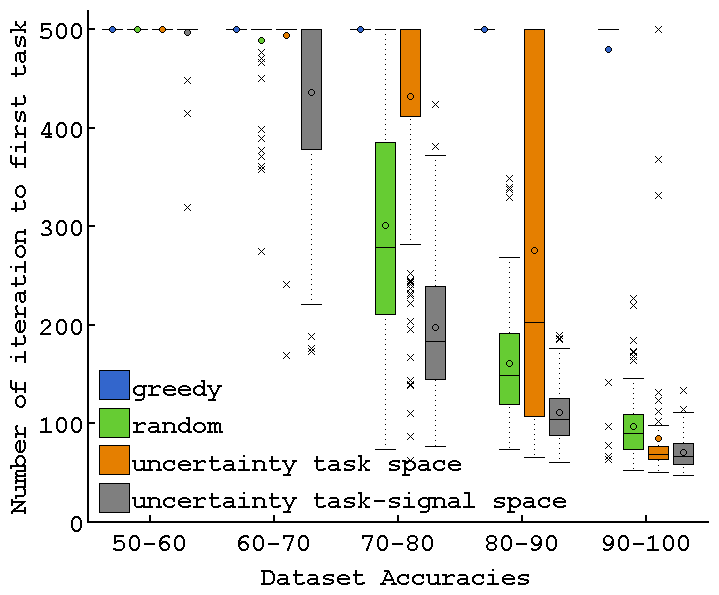
\includegraphics[width=\columnwidth]{\imgpath/plot_artificial_planning}
      \caption{Number of steps to complete first task, comparison of different exploration methods with 30 dimensional artificial data. When learning from scratch, planning upon uncertainty in both task and signal space performs better than relying only on task uncertainty. Greedy action selection rarely disambiguates between hypothesis.}
    \label{fig:planning}
\end{figure}


\paragraph{Dimensionality}

Figure \ref{fig:firstArtificial} compares the number of steps (with maximum values of 500 steps) needed to identify the first task when learning from scratch with different dimensionality of datasets. As can be seen, the convergence speed is only slightly affected by the features dimensionality. On the other hand, the dataset quality (measured in terms of their associated ten-fold accuracies) is the main cause of performances decay. Furthermore, for those datasets with accuracies between $60\%$ and $70\%$, the system is not able (on average) to learn the task after 500 steps.

\begin{figure}[!h]
  \centering
      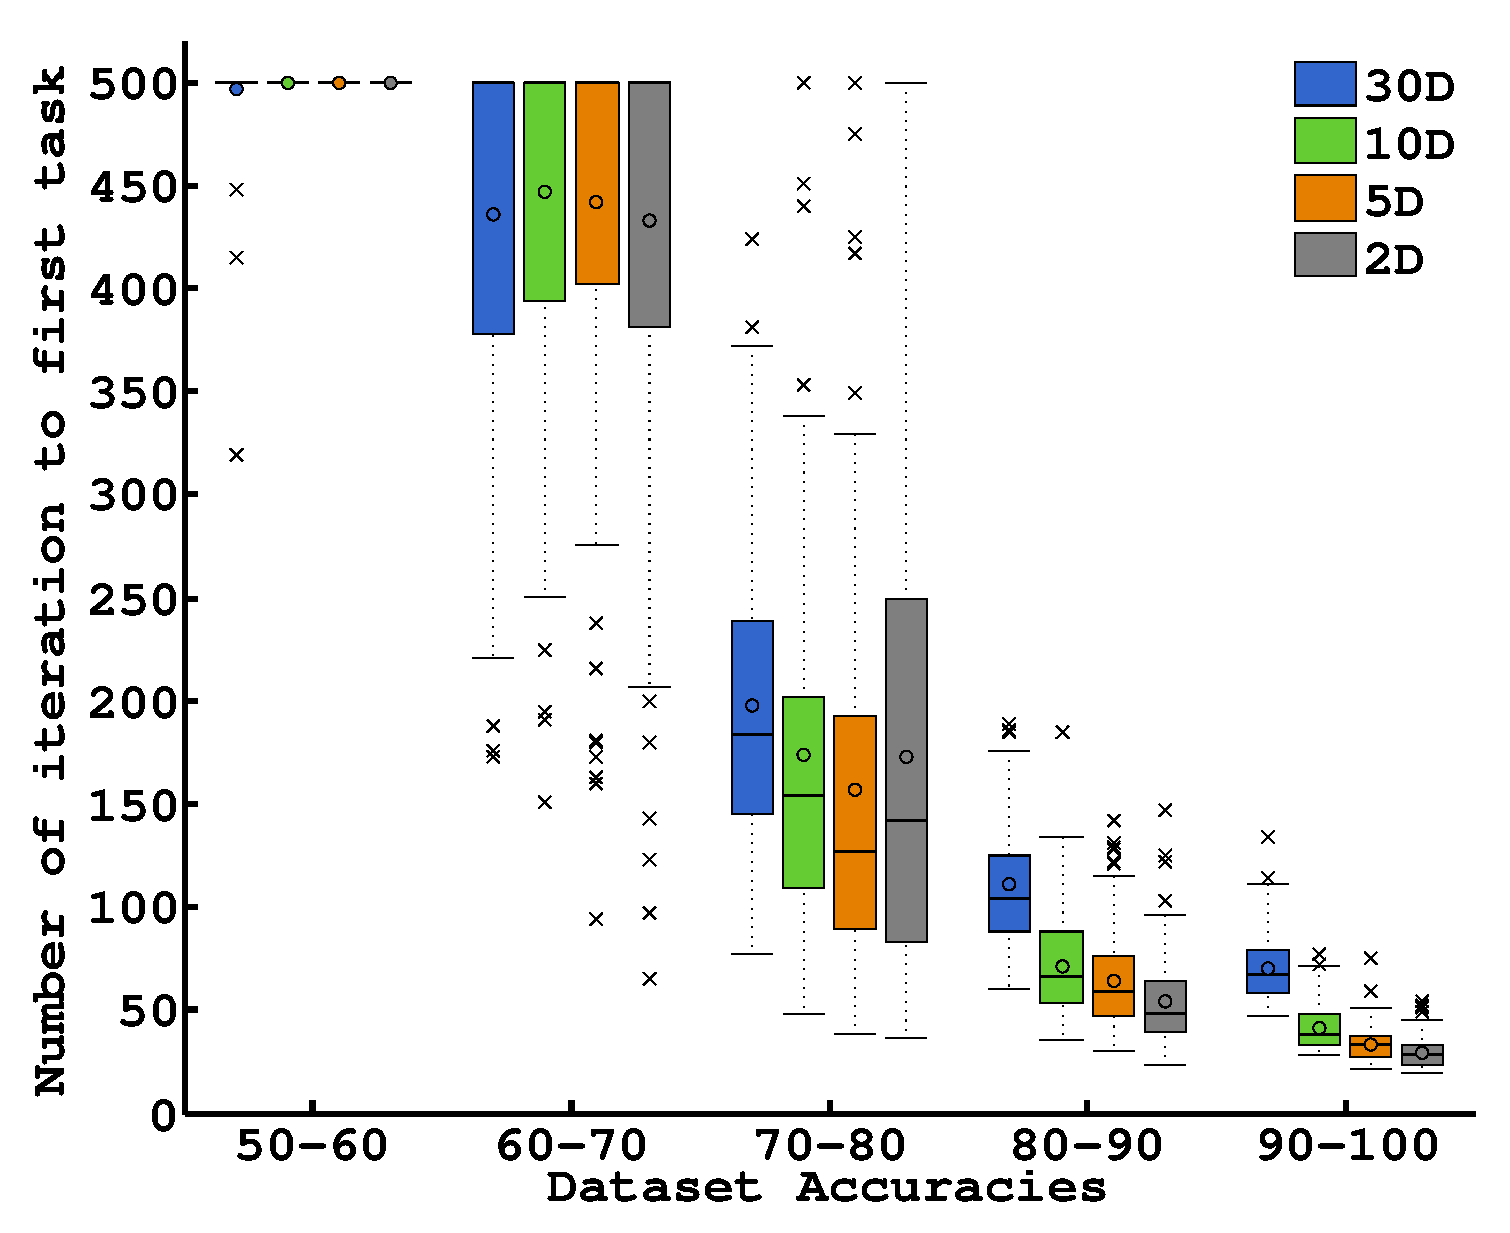
\includegraphics[width=\columnwidth]{\imgpath/plot_artificial_firstconf}
      \caption{Number of steps to complete first task using artificial data. Under 60 percent accuracy, the confidence threshold cannot be reached in 500 steps. The dataset qualities, more than their dimensionality, impact the learning time.}
      \label{fig:firstArtificial}
\end{figure} 

Once one task is completed, a new one is selected randomly. Figure \ref{fig:nCorrectArtificial} compares the number of tasks that can be achieved in 500 steps. As expected, the lower the quality of the data, the less number of task can be completed. On the other hand, with accuracies higher than $90\%$ dataset quality we can achieve more than 30 tasks on average. 

\begin{figure}[!h]
    \centering
    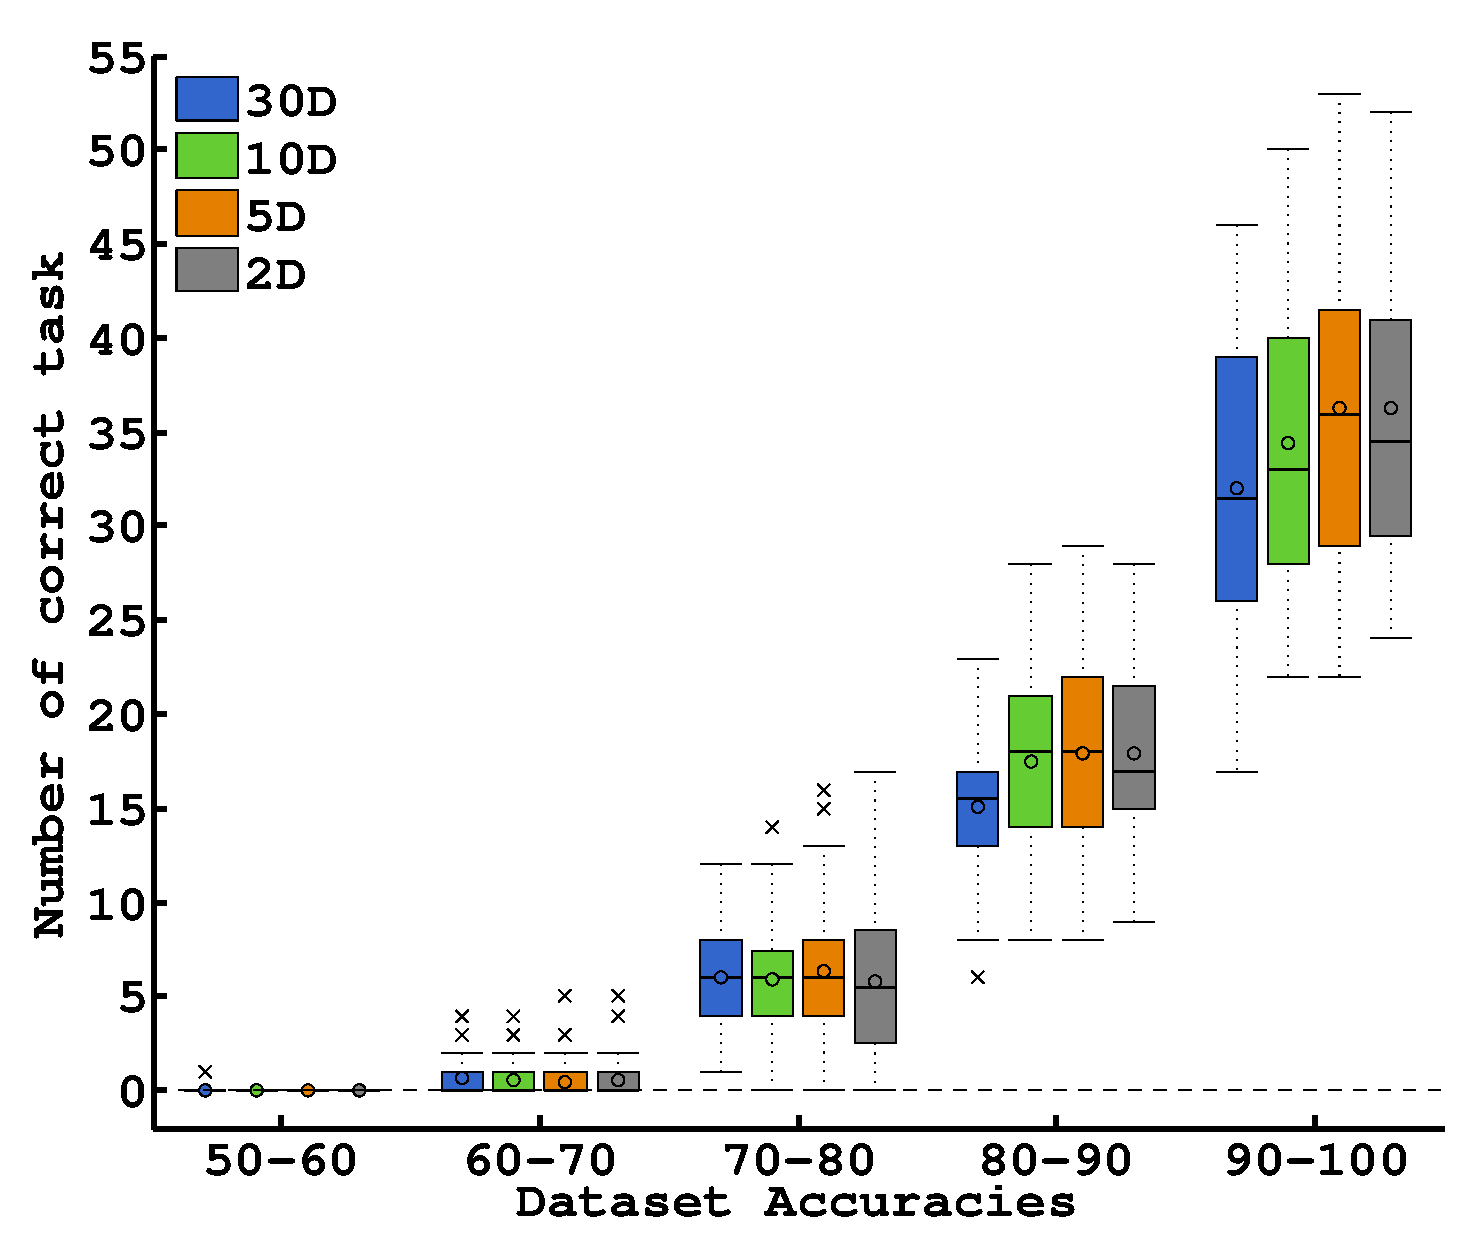
\includegraphics[width=\columnwidth]{\imgpath/plot_artificial_nCorrect}
    \caption{Number of tasks correctly achieved in 500 steps, artificial data. Quality of dataset impacts the number of task identified in 500 steps, more evidence should be collected to reach the confidence threshold.}
    \label{fig:nCorrectArtificial}
\end{figure} 

An important aspect of the proposed learning approach was that the first task learned was always the correct one. We reported only 9 erroneous estimations across all 900 artificial simulated experiments (5 in the 70-80 group and 4 in the 80-90 group).

\subsection{EEG datasets and comparison with calibration method}

\paragraph{Example}
Figure \ref{fig:sequence} shows one particular run of 500 steps comparing our self-calibration method with a calibration procedure of 400 steps. The two independent runs use as real EEG dataset with $80\%$ ten-fold classification accuracy. As our algorithm is operational from the first step, it can estimate the real task when sufficient evidence has been collected. On the other hand, a calibration approach collects signal-label pairs for a fixed number of steps and use the resulting classifier without updating it. This provokes that, during the calibration phase, no tasks can be learned, substantially delaying the user's online operation.

\begin{figure}[!h]
\centering
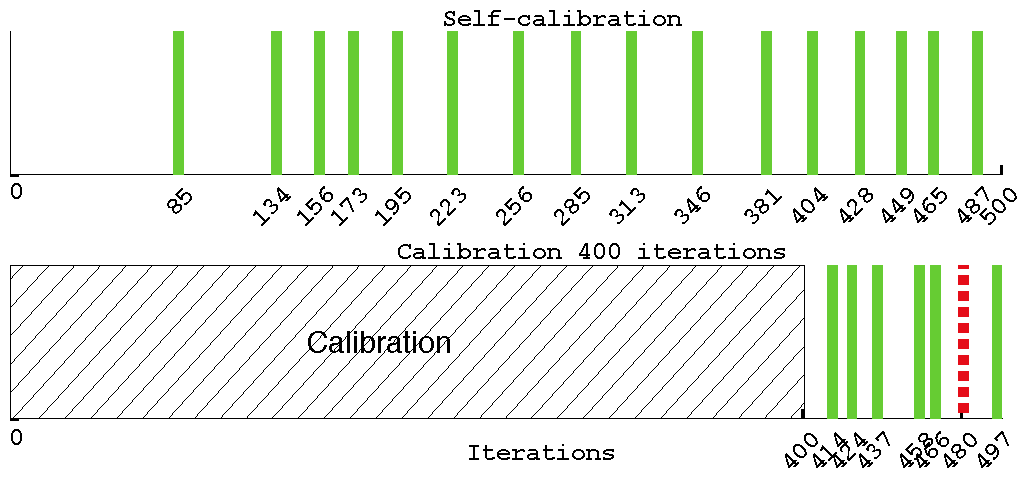
\includegraphics[width=\columnwidth]{\imgpath/plot_the_aaai_sequence}
\caption{Time-line of one run from EEG dataset of $80\%$ ten-fold classification accuracy, self-calibration (top) versus 400 steps calibration (bottom). Green (filled) and red (dashed) bars represents respectively correct and incorrect task achievement. The proposed self-calibration method allow to reach a first task faster than would take a calibration procedure.}
\label{fig:sequence}
\end{figure} 



Figure \ref{fig:sequence_evolution} shows the evolution of classification rate between our self-calibration method with a calibration procedure of 400 steps. As our method assigns different labels to each new teaching signal, the resulting classifiers have different performances, which help identifying the correct task. Once a task is identified (e.g.\ step 85 and 134), the corresponding labels are taken as ground truth, and all classifiers will have the same accuracies. As the agent starts exploring again the environment to estimate the new tasks, all the classifiers expect the true one will start to have worse accuracies again.

\begin{figure}[!h]
\centering
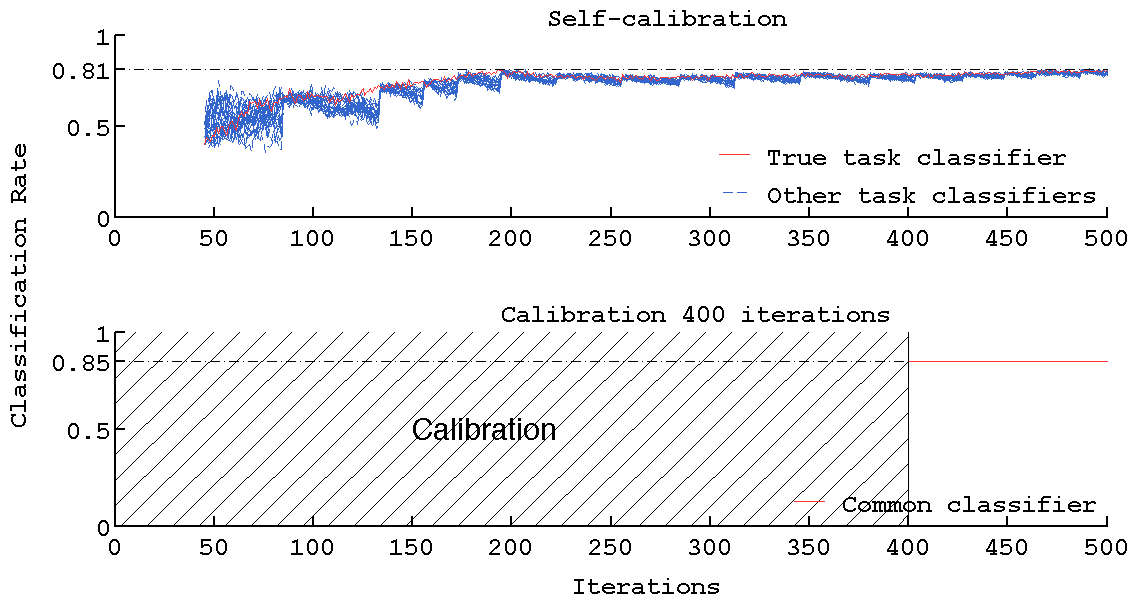
\includegraphics[width=\columnwidth]{\imgpath/plot_evo_classification_rate}
\caption{Evolution of classification rate of one run from EEG dataset of 83 percent accuracy, self-calibration (top) versus 400 steps calibration (bottom). On top, the red line represented the classifier corresponding the successive tasks taught by the user, the dashed blue one represent all others tasks. Our method updates classifiers every steps.}
\label{fig:sequence_evolution}
\end{figure} 

\paragraph{Time to first task}

Figure \ref{fig:firstEEG} shows the results per group of dataset. Our algorithm allows to complete the first task without errors and in a fair amount of iteration.  For our method, the learning time is strongly correlated with the dataset quality. However calibration methods, which do not update their classifier once calibrated, identify more tasks incorrectly.

\begin{figure}[!h]
\centering
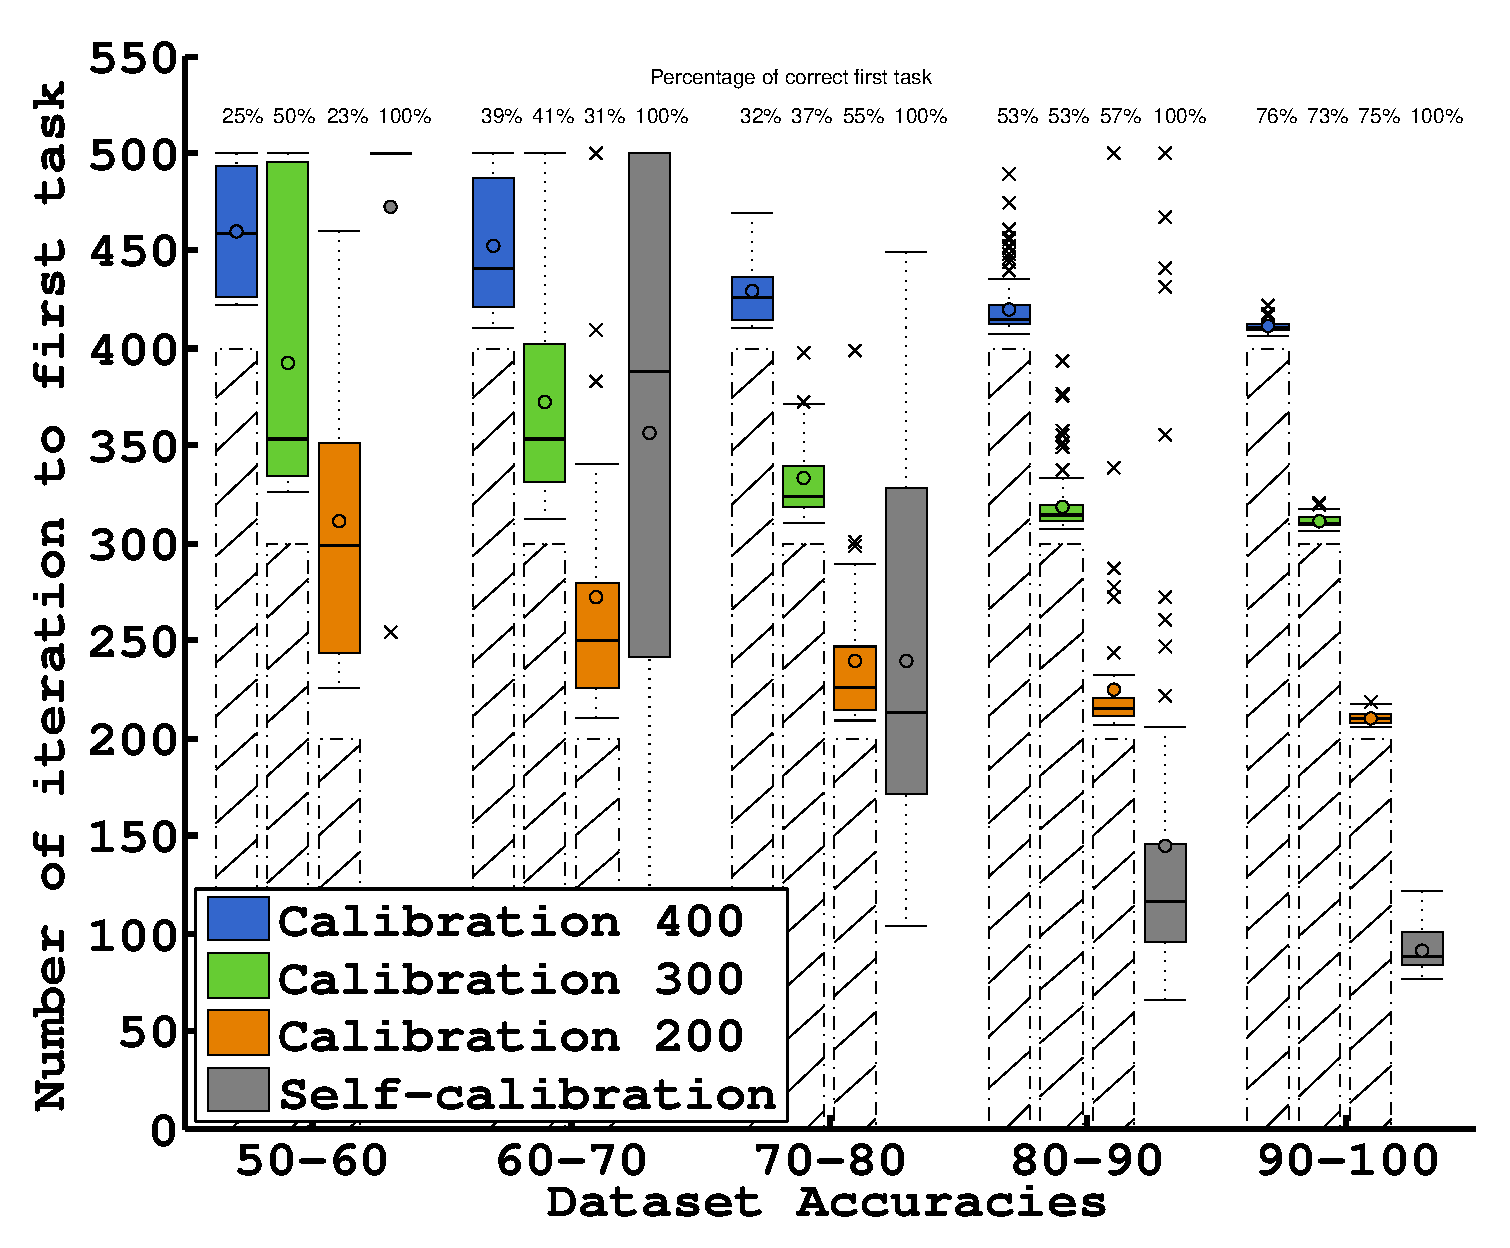
\includegraphics[width=\columnwidth]{\imgpath/plot_EEG_calib_firstconf}
\caption{Number of steps to complete first task with EEG data. The method scale well to EEG data. Contrary to the standard calibration approaches, we do not make mistakes with low quality datasets.}
\label{fig:firstEEG}
\end{figure} 

We can identify two main differences between our method and the usual calibration procedure for this kind of BCI experiments:
\begin{enumerate}
\item \textbf{Positive/Negative percent ratio of training examples}. Following the literature \cite{chavarriaga2010learning, iturrate2013task} we used a 80/20 percent ratio. Table \ref{tab:correctLabelRatio} shows the positive/negative ratio obtained following our planning method. The ratio we obtain is more balanced, resulting in classifiers with better properties. However a 50/50 percent ratio may lead to practical problems during online real world experiments and should be studied in more details, see open questions in section \ref{sec:conclusion}.
\item \textbf{Online update of multiple classifiers.} Our method integrates new data at every step whose label can differ between task hypothesis. For incorrect task hypothesis, the associated label can be incorrect and decrease the performance of the associated classifier, see figure \ref{fig:planningExplained}c. This dynamic can be observed in figure \ref{fig:sequence_evolution} where classifiers associated to incorrect tasks (in blue) have lower estimated accuracies than the correct one (in red). As a result our algorithm makes different predictions and updates for each hypothesis.
\end{enumerate}

\begin{table}
\begin{tabular}{c c c}
Dataset Accuracies & Self-calibration & Calibration \\ \hline
50-60 & 0.48 (0.02) & 0.8 (0) \\
60-70 & 0.50 (0.03) & 0.8 (0) \\
70-80 & 0.53 (0.03) & 0.8 (0) \\
80-90 & 0.57 (0.03) & 0.8 (0) \\
90-100 & 0.59 (0.01) & 0.8 (0) \\
\end{tabular}
\caption{Mean ratio of positive examples in training dataset (standard deviation shown in parenthesis). Calibration procedure for ErP EEG signal usual account for a 80 percent ratio of positive examples. However when following our method we collect as many positive than negative examples, see discussion in section \ref{sec:conclusion}.}
\label{tab:correctLabelRatio}
\end{table}

\begin{figure}[!h]
\centering
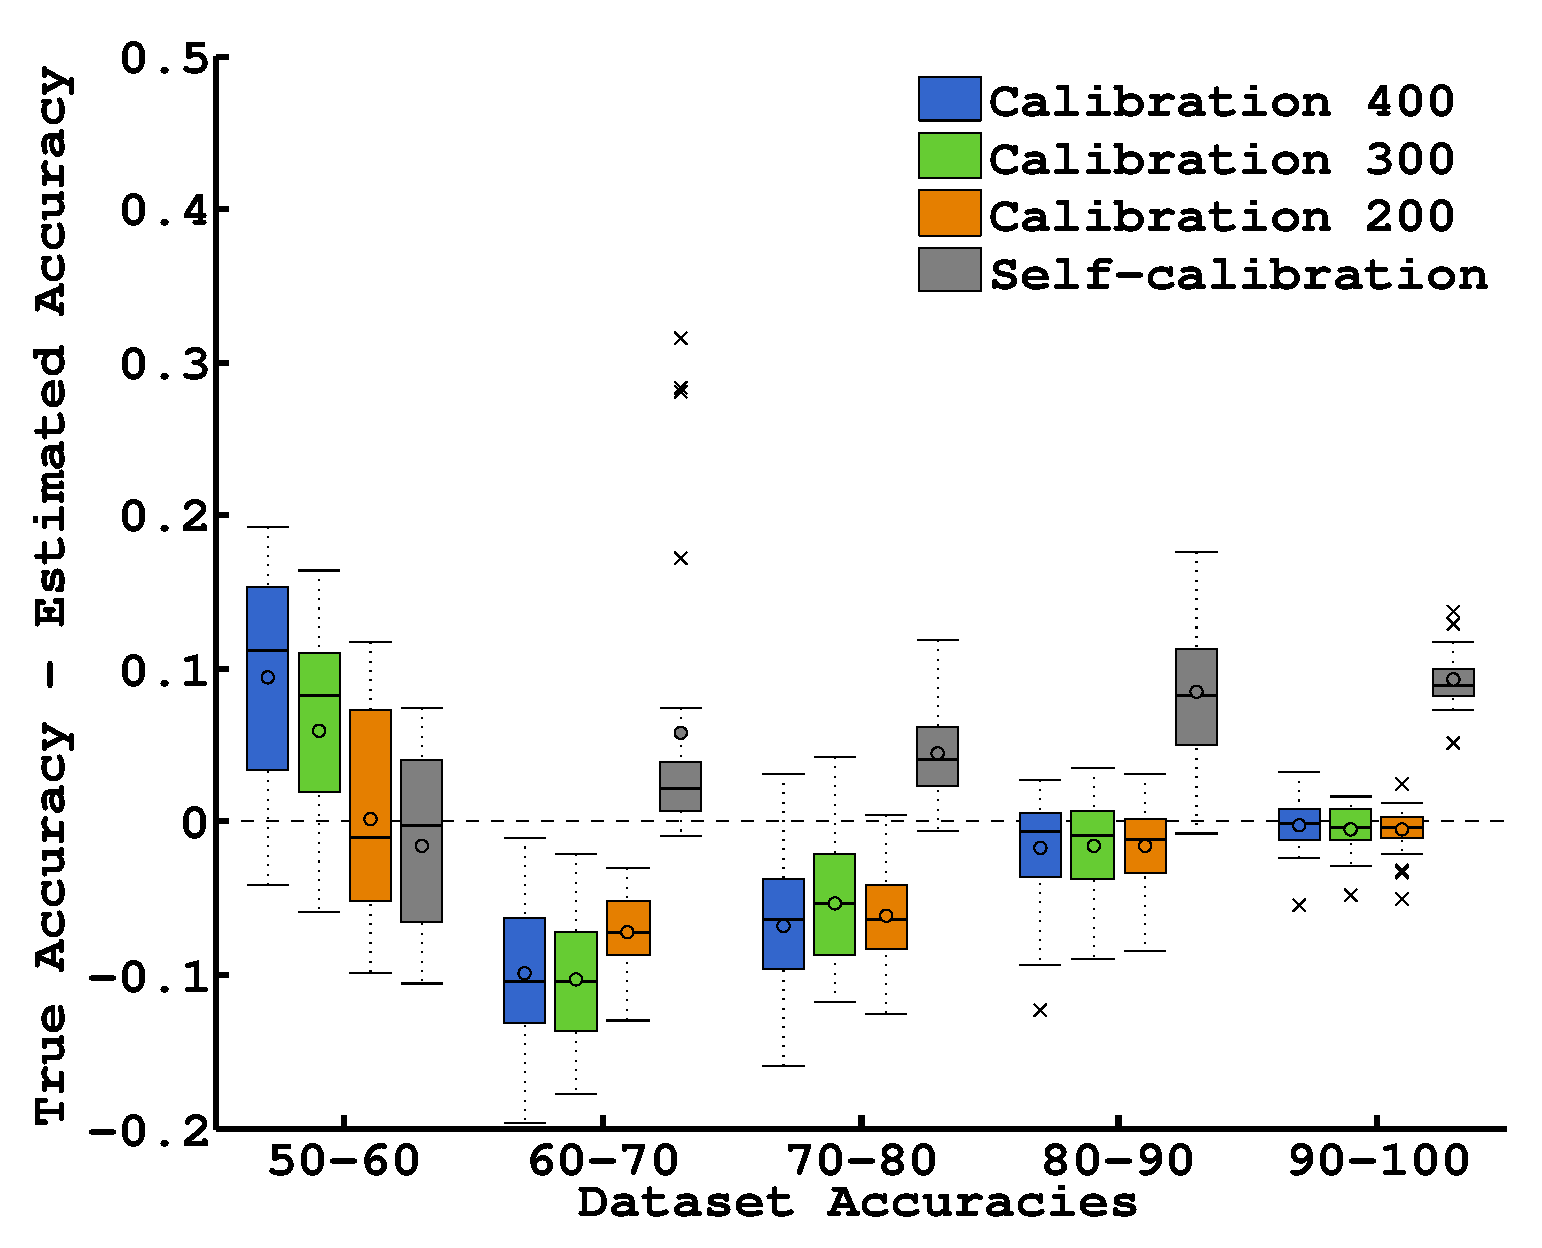
\includegraphics[width=\columnwidth]{\imgpath/plot_explaination_for_calib_failure}
\caption{Difference between true accuracy and estimated accuracy. True accuracy is the performance of the classifier on the unused data. Estimated accuracy is the 10 fold cross validation performance of the classifier on collected data. A negative(positive) value indicates the classifier is over(under)-estimating its performance. Calibration methods tend to produce over-confident classifiers, certainly due to the biased positive to negative training example ratio, see table \ref{tab:correctLabelRatio}.}
\label{fig:calibFail}
\end{figure}

\paragraph{Cumulative performances}

Figure \ref{fig:nCorrectEEG} compares the number of tasks that can be achieved in 500 steps. With 90\% and more dataset quality we can achieve about 20 tasks on average. The results are consistent with artificial dataset analysis.

\begin{figure}[!h]
\centering
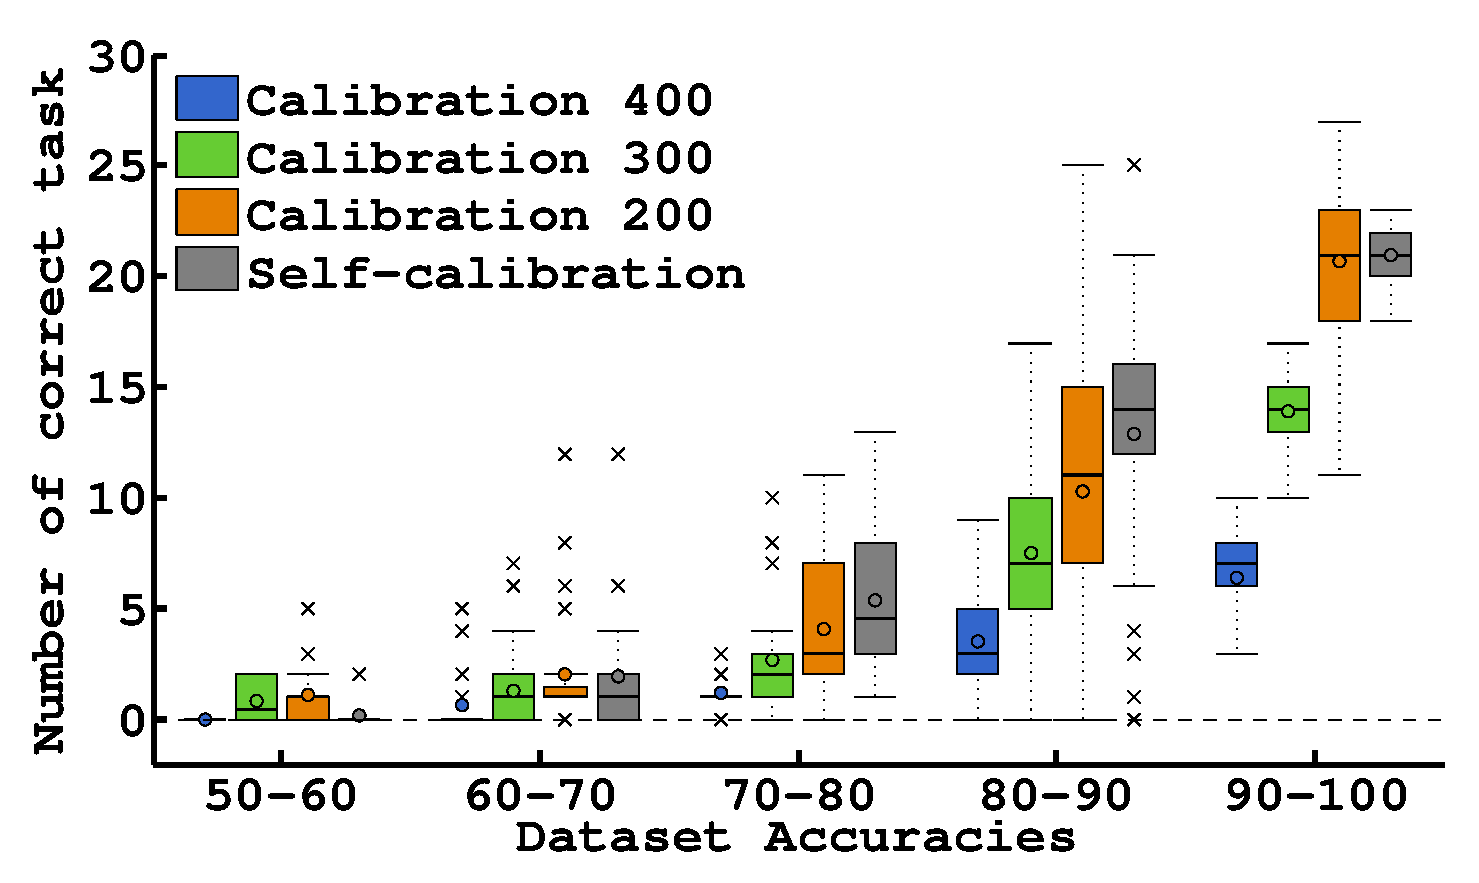
\includegraphics[width=\columnwidth]{\imgpath/plot_EEG_calib_nCorrect}
\caption{Number of task correctly achieved in 500 steps with EEG data. Calibration methods can not complete a significant number of task as most the time is spent on calibration.}
\label{fig:nCorrectEEG}
\end{figure} 

The calibration methods can not complete many task as a significant amount of iteration was used for calibrating the system. A calibration of 200 steps makes as many good estimation than our method, but it also makes many wrong estimation, see figure \ref{fig:nWrongEEG}. For calibration methods, the less time spent on calibration, the poorer the classifier which implies more mistakes.

\begin{figure}[!h]
\centering
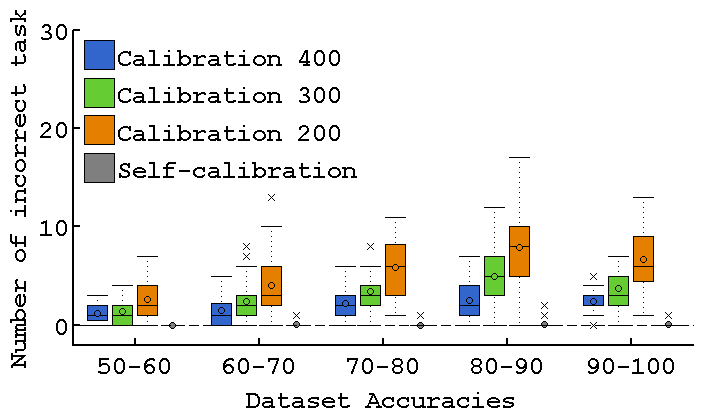
\includegraphics[width=\columnwidth]{\imgpath/plot_EEG_calib_nWrong}
\caption{Number of task incorrectly achieved in 500 steps with EEG data. Calibration methods, which do not update their models once calibrated, make more errors.}
\label{fig:nWrongEEG}
\end{figure}

\paragraph{Last 100 iterations performances}

Figure \ref{fig:nCorrectEEG_last100} compares the number of task that can be achieved during the last 100 steps with EEG data. With 80-90\% dataset quality, all methods achieve an average success rate of one task every 20 steps. However calibration methods, which do not update their models once calibrated, make more mistakes (see figure \ref{fig:nWrongEEG_last100}).

\begin{figure}[!h]
\centering
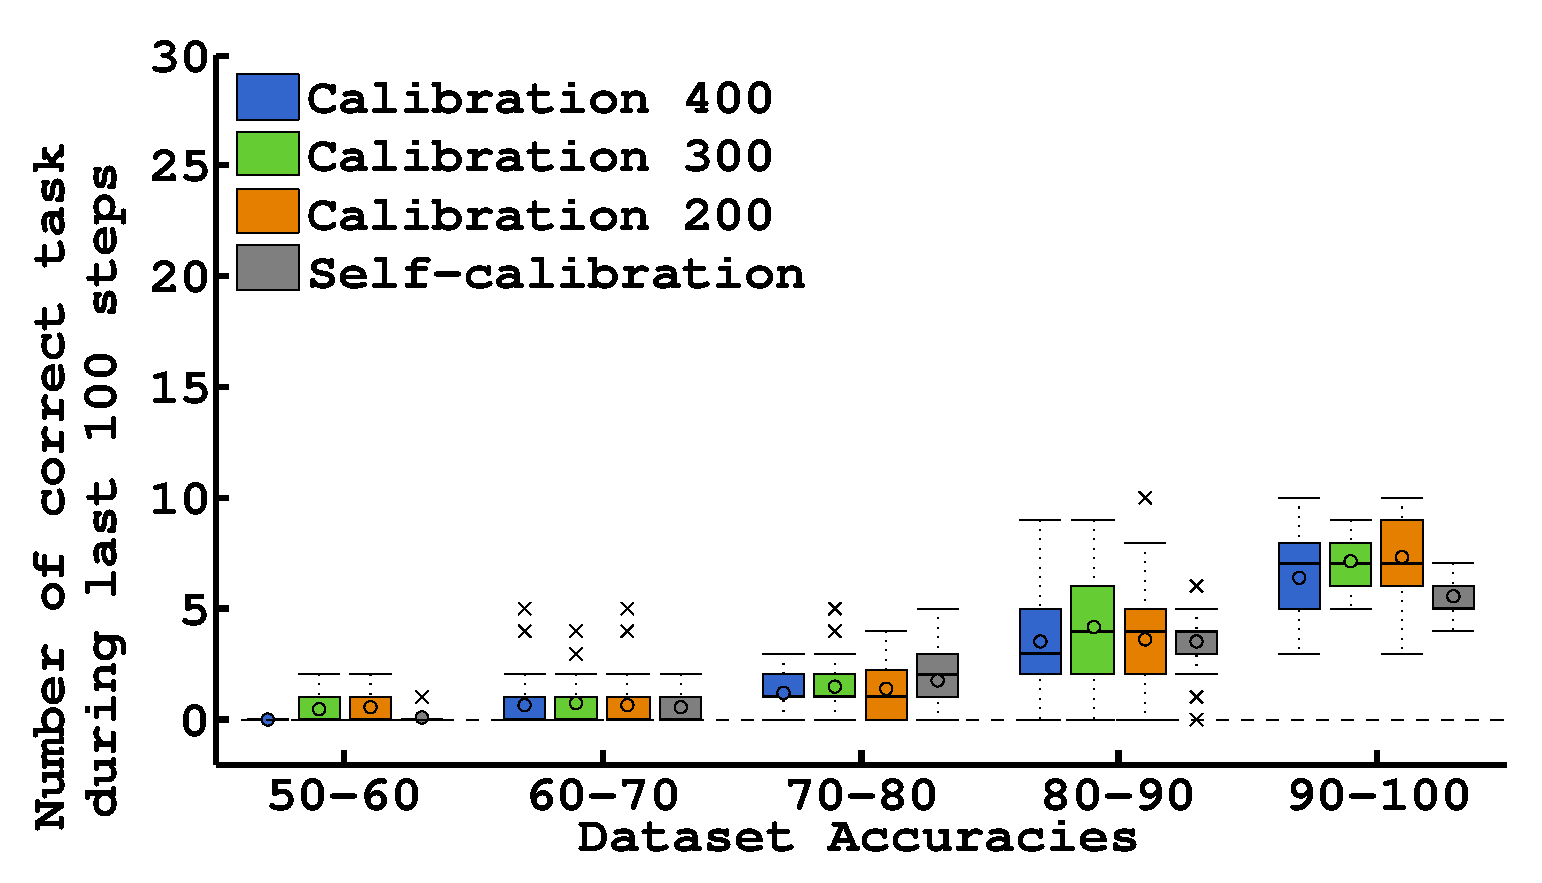
\includegraphics[width=\columnwidth]{\imgpath/plot_EEG_calib_nCorrect_last100}
\caption{Number of task correctly achieved during the last 100 steps with EEG data. All methods have equivalent successful reaching rate.}
\label{fig:nCorrectEEG_last100}
\end{figure} 

\begin{figure}[!h]
\centering
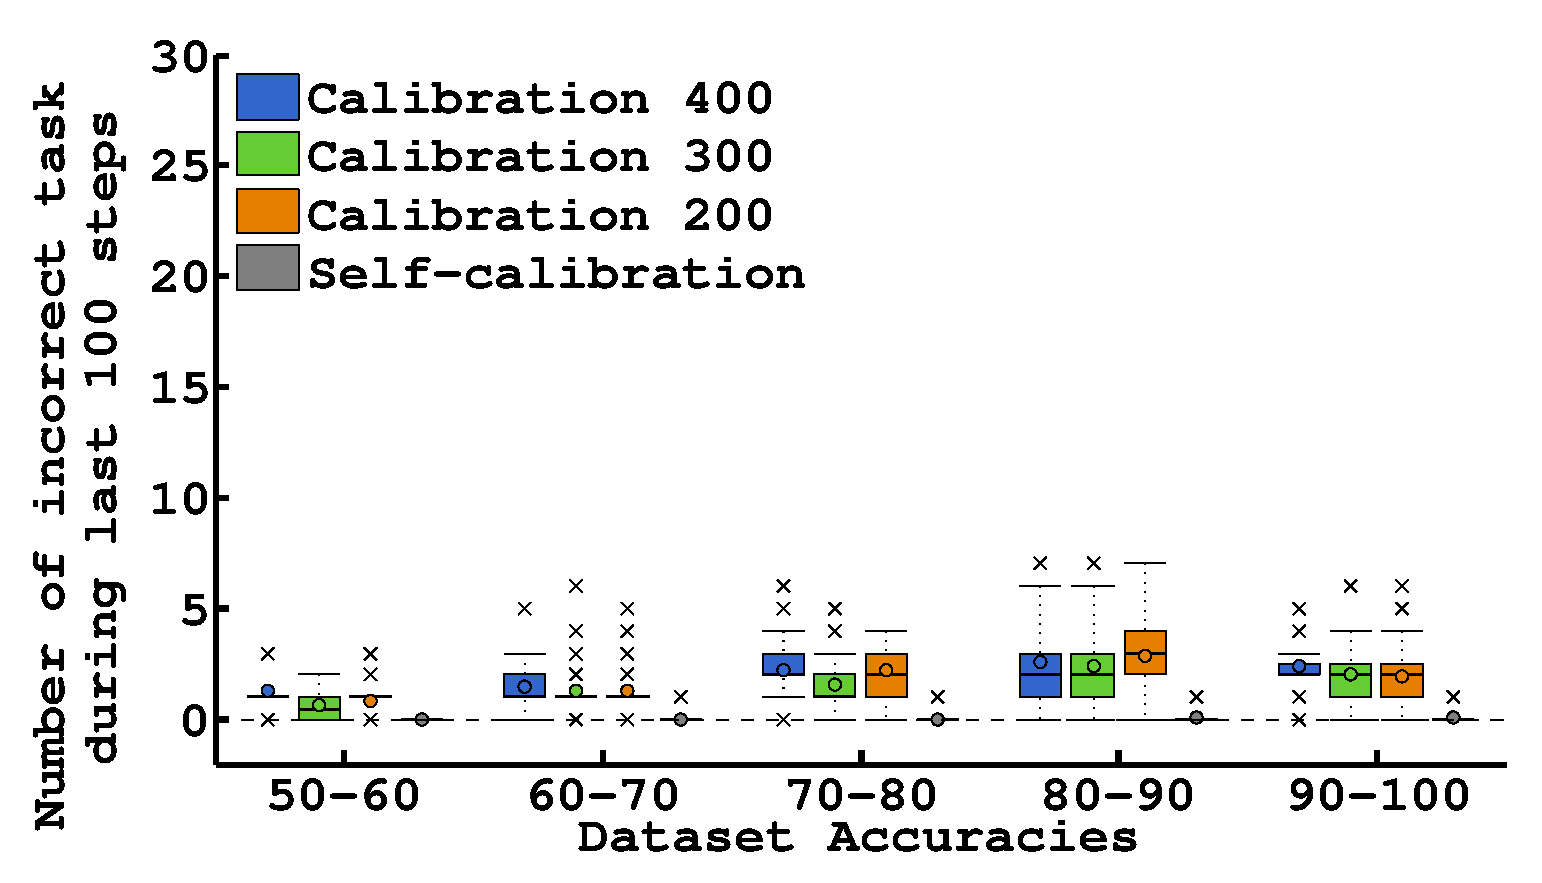
\includegraphics[width=\columnwidth]{\imgpath/plot_EEG_calib_nWrong_last100}
\caption{Number of task incorrectly achieved during the last 100 steps with EEG data. Calibration methods, which do not update their models once calibrated, make more errors.}
\label{fig:nWrongEEG_last100}
\end{figure} 

 shows the number of tasks identified with respect to the accuracy of the dataset, and the number of tasks incorrectly identified. Notice how the number of identified task is correlated to the quality of the dataset. Importantly, we were able to identify 15 to 20 tasks in 500 steps on good quality dataset without the need for a calibration procedure.


\begin{figure*}[t]
\centering
\begin{minipage}[t]{.65\columnwidth}
  \centering
          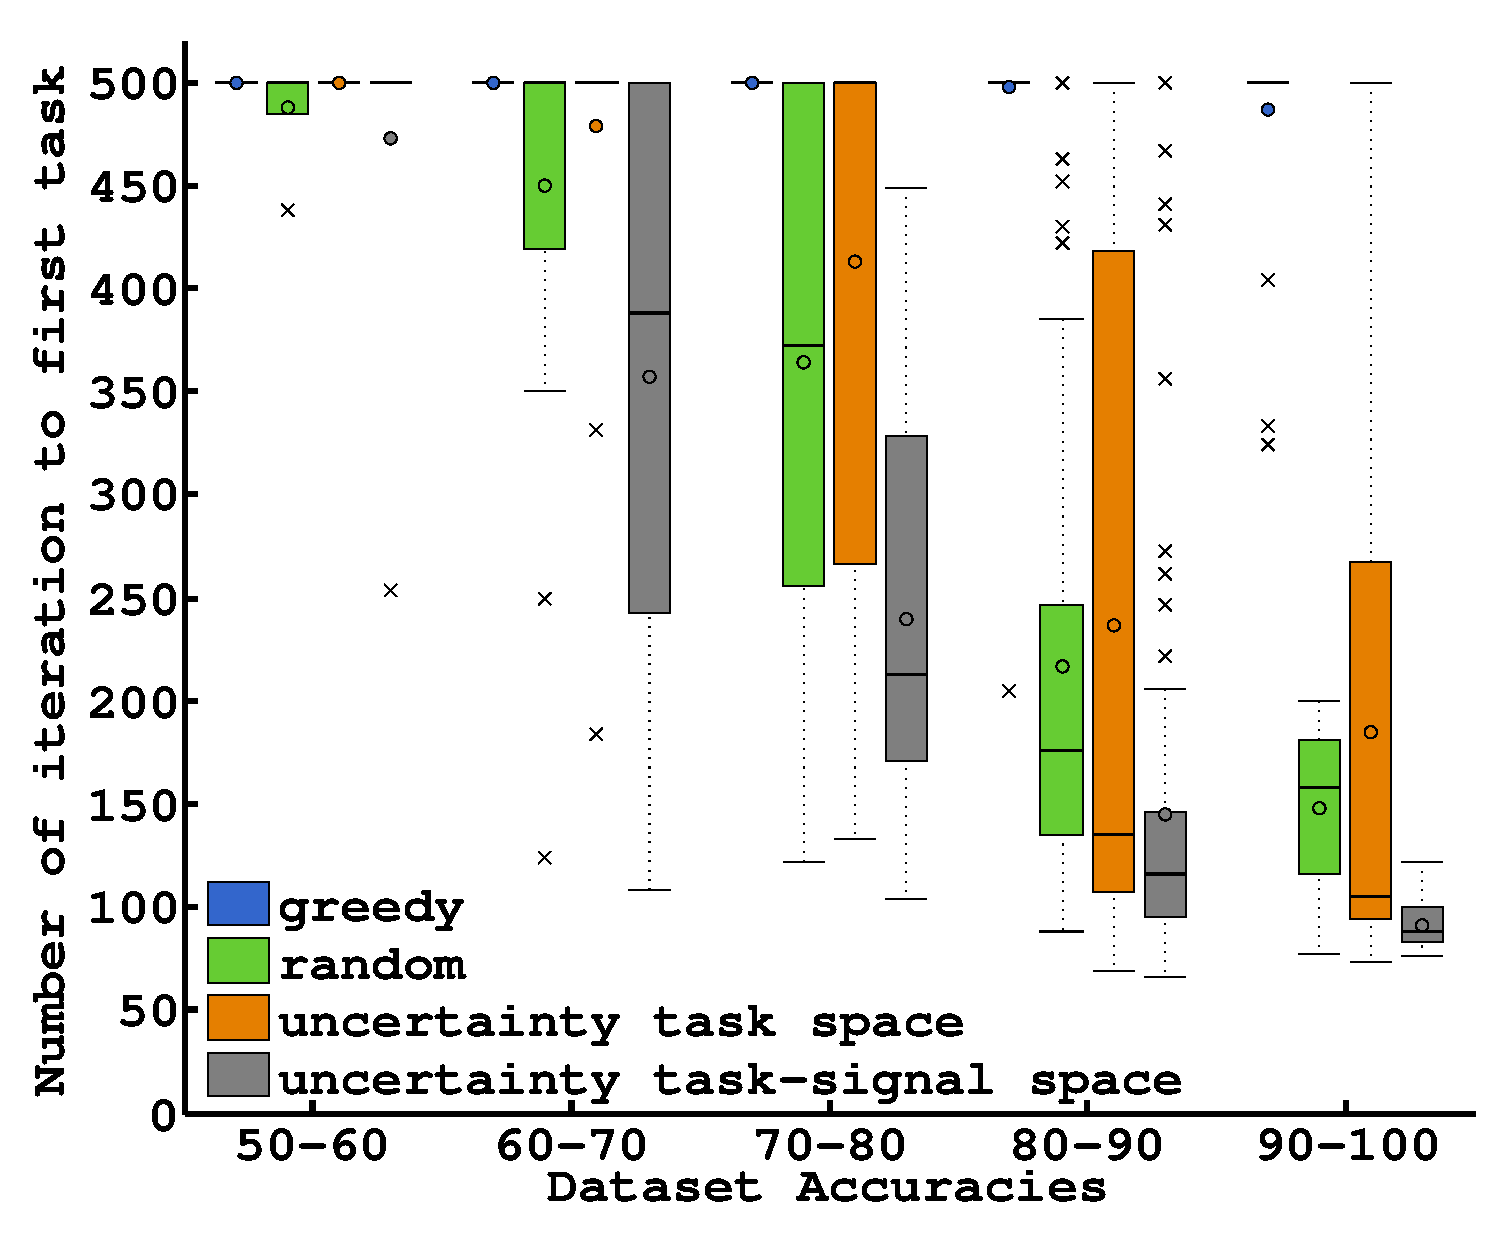
\includegraphics[width=\columnwidth]{\imgpath/plot_EEG_planning}
          \caption{\todo{this is the plot for EEG data, xp are running for artificial data}}
      \label{fig:planning}
\end{minipage}
\begin{minipage}[t]{.65\columnwidth}
  \centering
          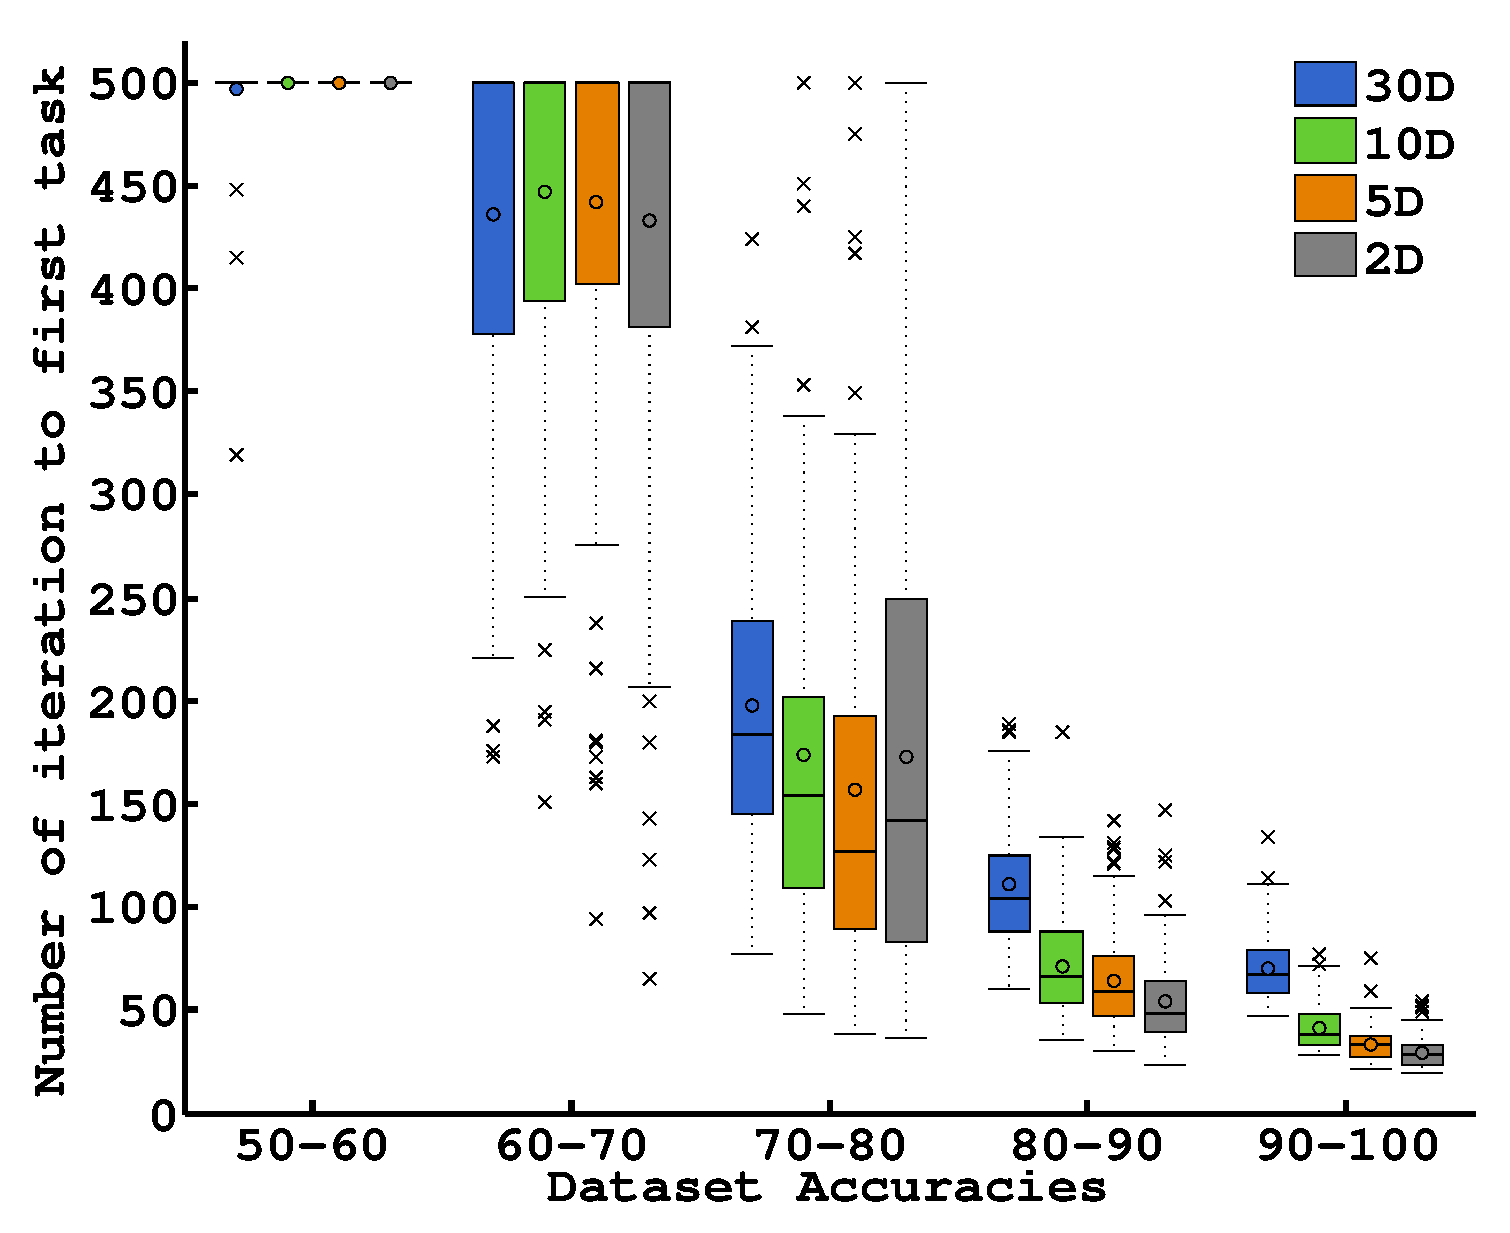
\includegraphics[width=\columnwidth]{\imgpath/plot_artificial_firstconf}
          \caption{Under 70 percent accuracy, the confidence threshold cannot be reached in 500 steps. The dataset qualities, more than their dimensionality, impact the learning time.}
          \label{fig:firstArtificial}
\end{minipage}    
\begin{minipage}[t]{.65\columnwidth}
  \centering
              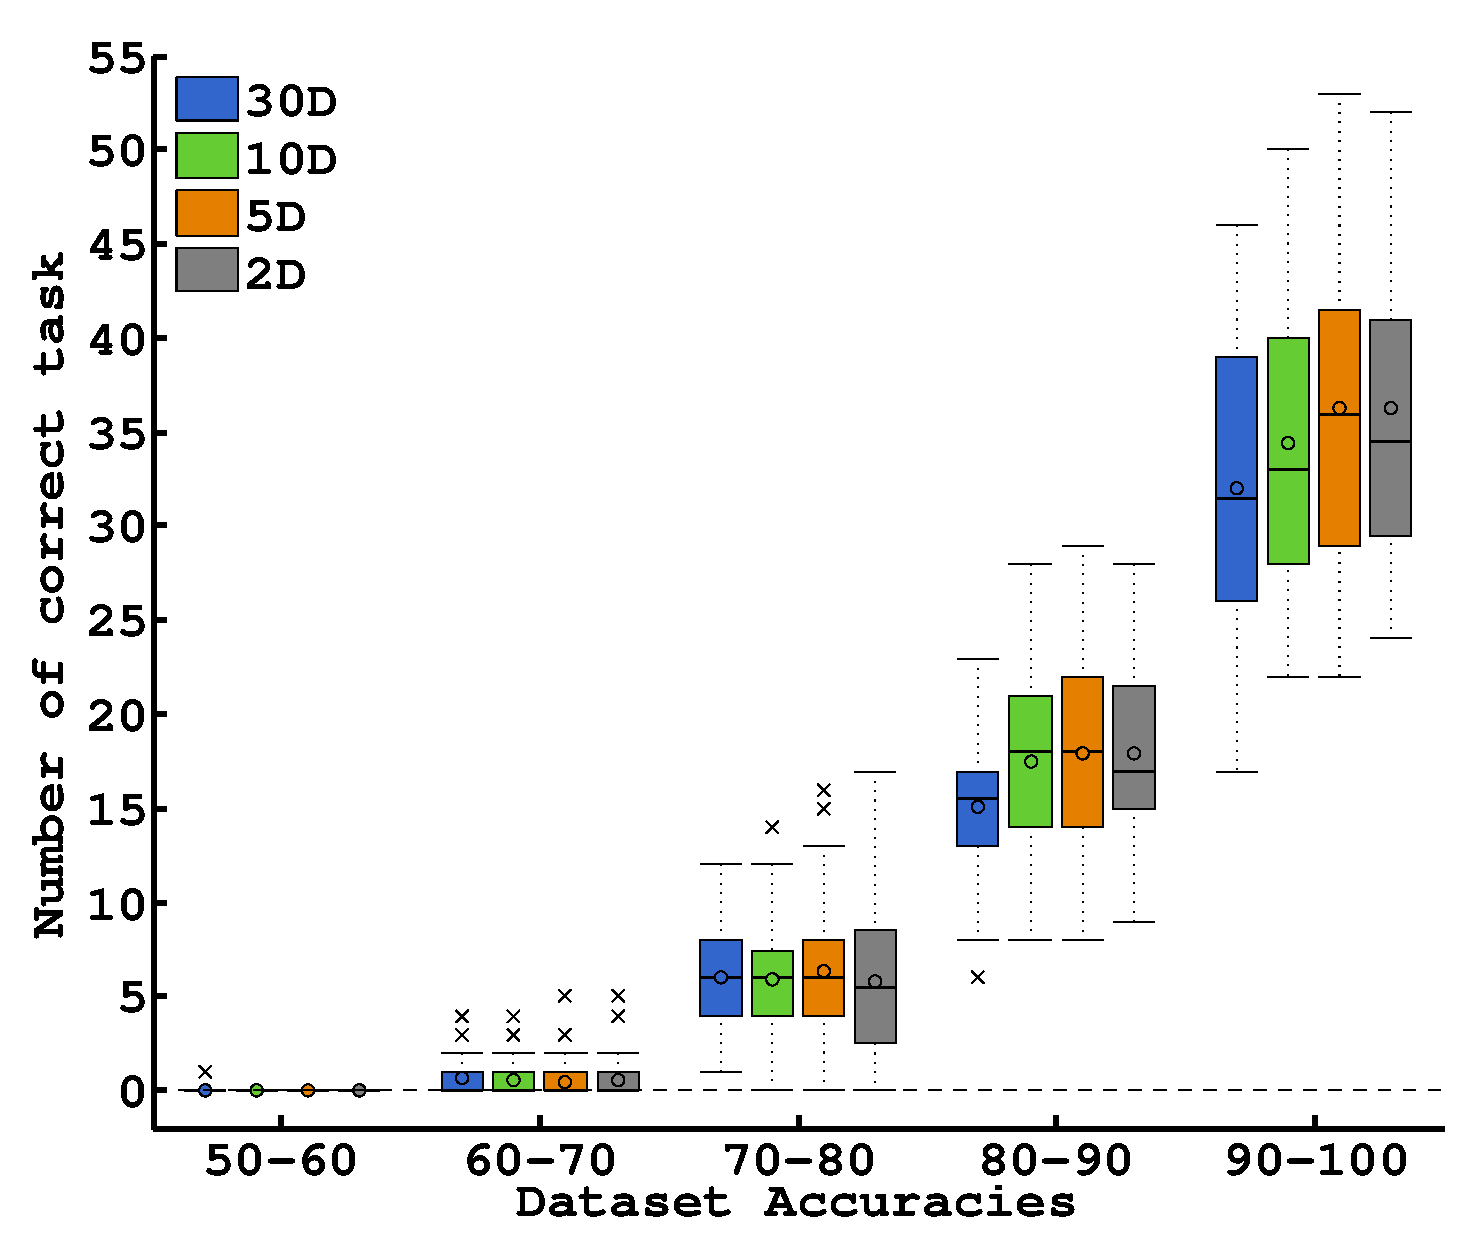
\includegraphics[width=\columnwidth]{\imgpath/plot_artificial_nCorrect}
          \caption{Quality of dataset impacts the number of task identified in 500 steps, more evidence should be collected to reach the confidence threshold.}
          \label{fig:nCorrectArtificial}
\end{minipage}
\end{figure*} 

\begin{figure}[t]
\centering
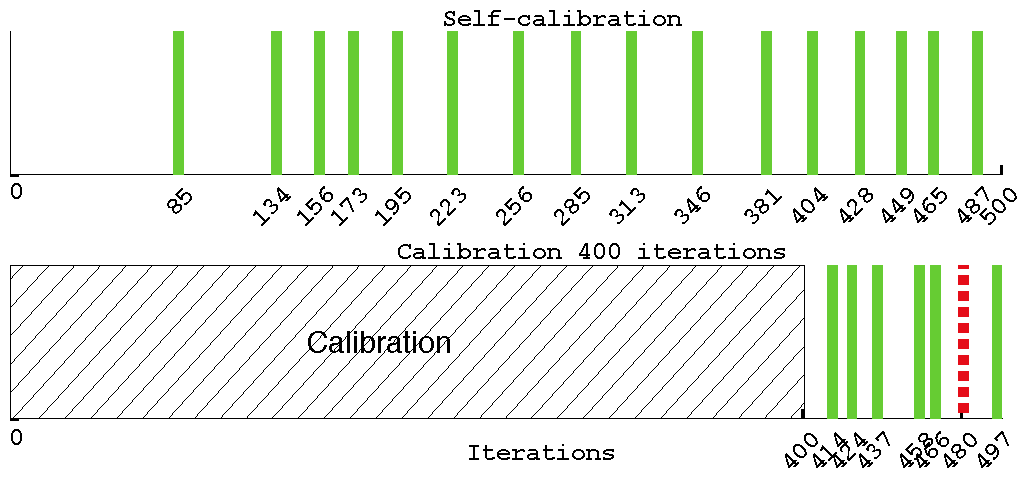
\includegraphics[width=\columnwidth]{\imgpath/plot_the_aaai_sequence}
\caption{The proposed self-calibration method allow to reach a first task faster, with performance increasing with time. One run from EEG dataset of 83 percent accuracy, self-calibration versus 400 steps calibration.}
\end{figure} 